% !TeX spellcheck = it
\documentclass[technote]{IEEEtran}
\IEEEoverridecommandlockouts
% The preceding line is only needed to identify funding in the first footnote. If that is unneeded, please comment it out.
\usepackage{cite}
\usepackage{amsmath,amssymb,amsfonts}
\usepackage{algorithmic}
\usepackage{graphicx}
\usepackage{textcomp}
\usepackage{xcolor}
\usepackage[italian]{babel}
\usepackage[utf8]{inputenc}
\usepackage{hyperref}
\usepackage{verbatimbox}
\usepackage{float}
\usepackage{listings}
\usepackage{subcaption} 

\def\BibTeX{{\rm B\kern-.05em{\sc i\kern-.025em b}\kern-.08em
    T\kern-.1667em\lower.7ex\hbox{E}\kern-.125emX}}
\begin{document}

\title{Classificazione di sottogeneri musicali tramite tecniche di text-mining}

\author{\IEEEauthorblockN{Lorenzo Mammana 807391}
\and
\IEEEauthorblockN{Gabriele Molteni 800900}
\and
\IEEEauthorblockN{Matteo Scarpone 800900}
}

\maketitle

\begin{abstract}
This document is a model and instructions for \LaTeX.
This and the IEEEtran.cls file define the components of your paper [title, text, heads, etc.]. *CRITICAL: Do Not Use Symbols, Special Characters, Footnotes, 
or Math in Paper Title or Abstract.
\end{abstract}

\begin{IEEEkeywords}
component, formatting, style, styling, insert
\end{IEEEkeywords}

\section{Introduzione}
Numerosi studi in letteratura sono stati effettuati riguardo la classificazione automatica di generi musicali sfruttando le liriche delle canzoni. Ci si aspetta che generi musicali diversi contengano tematiche e linguaggi molto differenti tra di loro e quindi la classificazione dovrebbe essere possibile. In questo studio si è deciso di verificare la possibilità di estendere questa analisi andando a valutare la possibilità di distinguere sottogeneri musicali di uno stesso genere. In particolare ci si è concentrati sull'analisi di sottogeneri della musica metal, questo tipo di musica presenta una enorme varietà di sottogeneri musicali, ciascuno con il proprio stile linguistico e le proprie tematiche.
La classificazione delle liriche è stata effettuata utilizzando tecniche di text-preprocessing e text-mining. Uno dei metodi più noti per la classificazione è quello basato su Latent Dirichlet Allocation (LDA), questo tipo di metodo permette di eseguire l'inferenza di \textit{Topic} all'interno di un testo in maniera non supervisionata.
Avendo a disposizione dati etichettati con uno o più sottogeneri si è utilizzato una versione più moderna di LDA, denomita LLDA (Labeled LDA) che permette di etichettare i \textit{topic} ottenendo una classificazione supervisionata.  

\section{Dataset}
Il dataset è stato costruito eseguendo lo scraping di due diversi siti web \href{http://www.darklyrics.com}{Darklyrics} e \href{https://www.metal-archives.com/}{Metal Archives}, il primo sito è una collezione di liriche, mentre il secondo è stato utilizzato per integrare le informazioni riguardo al genere degli artisti. 
La prima versione del dataset prodotta è composta da 259166 liriche, ogni lirica è composta dai seguenti campi:
\begin{itemize}
\item band - Il nome del gruppo compositore
\item album - L'album in cui è contenuta
\item year - L'anno di uscita
\item song - Il nome della canzone
\item lyrics - Le liriche della canzone
\item genre - Il genere o i generi della canzone
\item lang - La lingua della canzone
\end{itemize}
Il dataset estratto contiene numerosi campi mancanti come mostrato in tabella \ref{t_missing}:
\begin{table}[H]
\centering
\caption{Attributi mancanti e unici}
\begin{tabular}{|l|l|l|}
\hline
\textbf{Attributo} & \textbf{Mancanti} & \textbf{Valori unici} \\ \hline
band               & 0                 & 8456                  \\ \hline
album              & 11                & 26089                 \\ \hline
year               & 46                & 73                    \\ \hline
song               & 784               & 194215                \\ \hline
lyrics             & 17891             & 226154                \\ \hline
genre              & 55929             & 1694                  \\ \hline
lang               & 0             	   & 37                    \\ \hline
\end{tabular}
\label{t_missing}
\end{table}
Tutte le righe con attributi mancanti sono state eliminate dal dataset utilizzato per la classificazione finale. La lingua della lirica viene prodotta con un algoritmo in grado di calcolare la percentuale di appartenza di un testo ad una certa lingua, in tabella \ref{t_missing} il numero di \textit{lang} mancanti è nullo solamente perchè viene utilizzato il valore MISSING come placeholder. In tabella \ref{t_lang} viene invece mostrata la distribuzione delle prime dieci lingue contenute nel dataset.
\begin{table}[H]
\centering
\caption{Top 10 frequenza lingue}
\begin{tabular}{|l|l|}
\hline
\textbf{attributo} & \textbf{frequenza} \\ \hline
en                 & 0.796778           \\ \hline
MISSING            & 0.069033           \\ \hline
ro                 & 0.041854           \\ \hline
de                 & 0.025347           \\ \hline
es                 & 0.019949           \\ \hline
fi                 & 0.007833           \\ \hline
pt                 & 0.005483           \\ \hline
fr                 & 0.005336           \\ \hline
sv                 & 0.004460           \\ \hline
no                 & 0.004121           \\ \hline
\end{tabular}
\label{t_lang}
\end{table}
Per la classificazione finale sono state mantenute esclusivamente le liriche in lingua inglese, le altre lingue sono troppo poco frequenti per poter essere utilizzate e sarebbero un fattore confondente troppo grande per gli algoritmi di classificazione.
La rimozione delle liriche mancanti o non in inglese riduce il numero di righe a 200556.
\subsection{Gestione del genere musicale}
Come si vede in tabella \ref{t_missing} il numero di generi univoci presenti all'interno del dataset è estremamente elevato, questo è dovuto al fatto che i dati estratti tramite scraping non sono ben categorizzati, ma possono presentare leggere variazioni o ordinamenti differenti. Per poter rendere fattibile la classificazione è stata utilizzata la conoscenza del dominio per raggruppare i sottogeneri in macro-sottogeneri, in particolare la scelta è stata quella di fissare nove generi principali a cui vengono ricondotte tutte le liriche nle dataset. Questo introduce ovviamente un bias in quanto la categorizzazione è basata esclusivamente su conoscenza a priori riguardante il genere, senza essere influenzata dall'effettivo contenuto delle liriche. Un secondo bias è relativo al fatto che i generi sono associato al gruppo musicale e non al singolo album, ciò che accade nella realtà è che un artista produce album di diversi generi, mentre invece nel dataset questa distinzione non è evidente.\newpage
I nove generi proposti sono i seguenti:
\begin{itemize}
\item Rock
\item Heavy
\item Thrash
\item Power
\item Folk
\item Progressive
\item Death
\item Doom
\item Black
\end{itemize}
I generi sono stati selezionati in base alle pre-conoscenze degli autori in modo tale che possa essere stabilito un ordine tra di essi; nella lista precedente ogni genere è teoricamente contenuto all'interno dell'insieme composto dal genere successivo. Vengono prodotti due dataset utilizzati per il task di classificazione, il primo è un dataset multi-label, mentre il secondo utilizza l'ordinamento per associare una singola label come attributo di output. I dataset prodotti sono fortemente sbilanciati, il dataset multilabel può teoricamente rappresentare $ 2^9 - 1 = 511 $ generi diversi, nel dataset sono presenti solamente 110 di queste possibili combinazioni. Come mostrato in tabella \ref{t_multi_genres} sono solamente 18 i generi con frequenza superiore all'1\%, ci si aspetta quindi che la classificazione su questo dataset sarà particolarmente complicata.
\begin{table}[H]
\centering
\caption{Generi con frequenza superiore all'1\%}
\begin{tabular}{|l|l|}
\hline
\textbf{Generi}                    & \textbf{Frequenze} \\ \hline
\{Death Metal\}                    & 0.214409           \\ \hline
\{Black Metal\}                    & 0.097342           \\ \hline
\{Power Metal\}                    & 0.072505           \\ \hline
\{Thrash Metal\}                   & 0.063777           \\ \hline
\{Heavy Metal\}                    & 0.058732           \\ \hline
\{Death Metal, Thrash Metal\}      & 0.050035           \\ \hline
\{Doom Metal\}                     & 0.046568           \\ \hline
\{Death Metal, Doom Metal\}        & 0.037722           \\ \hline
\{Progressive Metal\}              & 0.031522           \\ \hline
\{Heavy Metal, Power Metal\}       & 0.031199           \\ \hline
\{Death Metal, Black Metal\}       & 0.027881           \\ \hline
\{Heavy Metal, Rock\}              & 0.024937           \\ \hline
\{Thrash Metal, Power Metal\}      & 0.019998           \\ \hline
\{Heavy Metal, Thrash Metal\}      & 0.019103           \\ \hline
\{Progressive Metal, Power Metal\} & 0.014146           \\ \hline
\{Doom Metal, Black Metal\}        & 0.012251           \\ \hline
\{Doom Metal, Heavy Metal\}        & 0.010021           \\ \hline
\end{tabular}
\label{t_multi_genres}
\end{table}
Nel caso singola-label il dataset rimane piuttosto sbilanciato, ma la classificazione dovrebbe essere nettamente più semplice da eseguire. Le frequenze sono mostrate in tabella \ref{t_single_genre}.
\begin{table}[H]
\centering
\caption{Frequenze generi singola label}
\begin{tabular}{|l|l|}
\hline
\textbf{Genere}   & \textbf{Frequenza} \\ \hline
Death Metal       & 47379              \\ \hline
Black Metal       & 28444              \\ \hline
Power Metal       & 21019              \\ \hline
Doom Metal        & 19413              \\ \hline
Thrash Metal      & 13341              \\ \hline
Rock              & 11101              \\ \hline
Heavy Metal       & 9454               \\ \hline
Progressive Metal & 8757               \\ \hline
Folk Metal        & 2060               \\ \hline
\end{tabular}
\label{t_single_genre}
\end{table}
\'E interessante notare l'andamento dei generi nel tempo, il dataset fornisce una buona copertura dei generi per anno, in particolare si vede, come è accaduto realmente, un aumento della "pesantezza" del genere musicale con il passare degli anni (Figura \ref{fig_genre_year}).


\begin{figure}[H]
\centerline{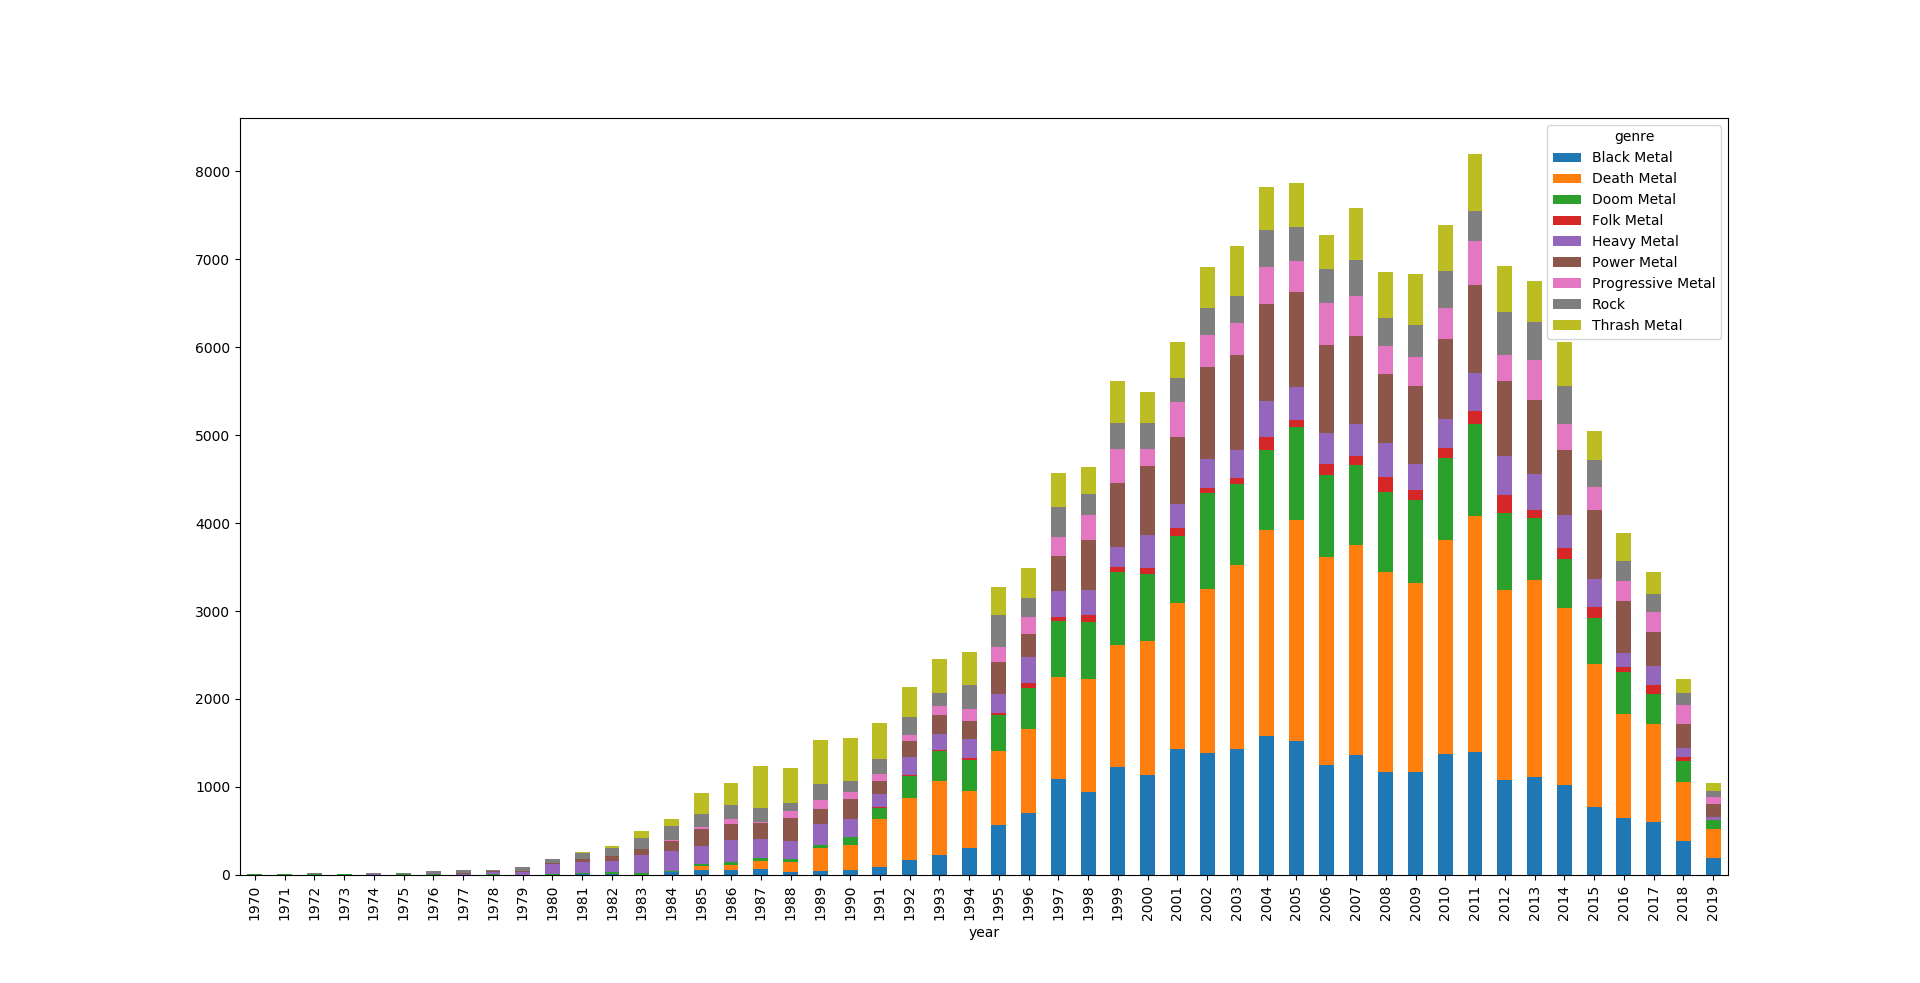
\includegraphics[width=0.5\textwidth]{images/genre_per_year_distribution}}
\caption{Distribuzione dei generi musicali negli anni}
\label{fig_genre_year}
\end{figure}

\section{Preprocessamento del testo}
Le liriche estratte inizialmente sono molto sporche, contengono punteggiatura, parole poco o troppo frequenti etc... Per poter eseguire una classificazione corretta è necessario procedere con un'operazione di filtraggio del testo per ottenere dei \textit{token} ben formati. Per farlo si è proceduto costruendo un workflow Knime utilizzato come wrapper per il codice Python, la scelta di utilizzare Python è dovuta al consumo estremamente elevato di risorse da parte di Knime sul dataset in questione, le operazioni che in Python richiedono pochi minuti con un consumo limitato di memoria in Knime necessitano di un numero estremamente più elevato sia di tempo che di memoria.
\begin{figure}[H]
\centerline{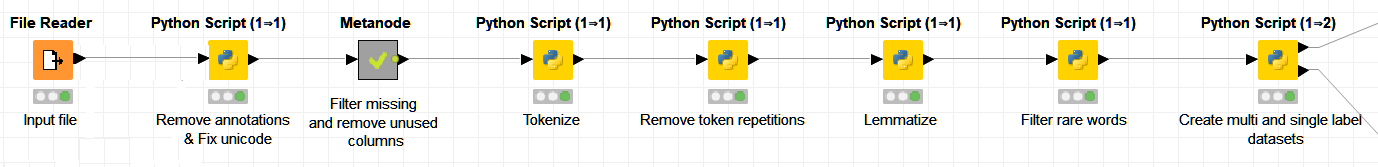
\includegraphics[width=1\columnwidth]{images/knime-text-prep}}
\caption{Workflow preprocessamento del testo in Knime}
\label{fig_knime_prep}
\end{figure}
\subsection{Tokenizzazione}
La tokenizzazione è stata eseguita con il package \textit{nltk} (Natural language toolkit), uno dei più utilizzati in questo ambito. Il primo passo è quello di separare ogni lirica nelle frasi che la compongono, questo viene ottenuto per mezzo di un modello supervisionato di \textit{Sentence boundary disambiguation} (SBD) preaddestrato su un insieme molto ampio di testi. L'applicazione di questo modello e la seguente rimozione della punteggiatura produce un risultato di questo tipo:

\begin{lstlisting}[basicstyle=\tiny]
  Searching the darkness. And emptineeess. I'm hiding away from the sun  
  ['Searching the darkness', 'And emptineeess', 'I m hiding away from the sun']  
\end{lstlisting}
Si procede poi all'estrazione vera e propria dei singoli token, questa viene eseguita tramite l'utilizzo di espressioni regolari, in particolare utilizzando il \textit{Penn Treebank}. Questo permette di rimuovere token troppo frequenti basati sulla grammatica inglese e risolvere le contrazioni di alcune parole. I token vengono poi convertiti in minuscolo, vengono rimossi i numeri e le parole più corte di tre caratteri.

\begin{lstlisting}[basicstyle=\tiny]
  ['Searching the darkness', 'And emptineess', 'I m hiding away from the sun']  
  ['searching', 'darkness', 'emptineeess', 'hiding', 'away', 'sun']
\end{lstlisting}
Viene poi eseguita la rimozione delle ripetizioni nelle parole, l'algoritmo utilizzato rimuove iterativamente le lettere multiple dai token e verifica su un dizionario se la parola esiste o meno, in modo tale da decidere se continuare l'eliminazione o fermarsi.
Si è proceduto verificando quali sono lo parole più frequenti per ogni genere, si nota che le dieci parole più frequenti sono piuttosto simili all'interno di ogni genere come visibile in tabella \ref{t_10_word}.

\begin{lstlisting}[basicstyle=\tiny]
  ['searching', 'darkness', 'emptineeess', 'hiding', 'away', 'sun']
  ['searching', 'darkness', 'emptines', 'hiding', 'away', 'sun']
\end{lstlisting}
In questo caso l'algoritmo sbaglia sulla parola \textit{emptiness} andando a rimuovere la seconda s. \\
Si è poi analizzata la frequenza dei token per genere, come visibile in tabella \ref{t_10_word} i primi dieci token di ogni genere sono piuttosto simili, questo è comunque corretto dato che i sottogeneri fanno tutti parte dello stesso insieme iniziale.
\begin{table}[H]
\centering
\caption{Top 10 parole frequenti per genere}
\resizebox{\columnwidth}{!}{
\begin{tabular}{|l|l|l|l|l|l|l|l|l|}
\hline
\textbf{Rock} & \textbf{Heavy} & \textbf{Thrash} & \textbf{Power} & \textbf{Folk} & \textbf{Progressive} & \textbf{Death} & \textbf{Doom} & \textbf{Black} \\ \hline
away          & got                  & death                 & away                 & blood               & away                       & blood                & away                & black                \\ \hline
got           & know                 & know                  & know                 & come                & eyes                       & death                & eyes                & blood                \\ \hline
know          & life                 & life                  & life                 & land                & know                       & eyes                 & know                & death                \\ \hline
life          & like                 & like                  & never                & life                & life                       & life                 & life                & eyes                 \\ \hline
like          & never                & never                 & night                & like                & like                       & like                 & like                & life                 \\ \hline
love          & night                & one                   & one                  & never               & never                      & never                & never               & night                \\ \hline
never         & one                  & see                   & see                  & night               & one                        & one                  & one                 & one                  \\ \hline
one           & see                  & time                  & time                 & one                 & see                        & see                  & see                 & see                  \\ \hline
see           & take                 & way                   & way                  & see                 & time                       & time                 & time                & time                 \\ \hline
time          & time                 & world                 & world                & time                & world                      & world                & world               & world                \\ \hline
\end{tabular}
}
\label{t_10_word}
\end{table}
In totale vengono estratti 209780 token differenti.
\subsection{Lemmatizzazione}
Per ridurre ulterirormente il numero di token estratti si è proceduto eseguendo il loro stemming, cercando quindi di ricondurre token simili alla loro radice comune. \'E stato utilizzato il \textit{LancasterStemming}, un tipo di stemming molto "aggressivo" che riduce di molto la lunghezza dei token, la scelta dell'utilizzo di questo algoritmo è dovuta principalmente alla grande dimensione del dataset, si è deciso di sacrificare leggermente la leggibilità dei dati per ottenere un aumento di velocità nell'esecuzione degli algoritmi. Sulla frase mostrata in precedenza l'algoritmo produce i seguenti risultati:
\begin{lstlisting}[basicstyle=\tiny]
  ['searching', 'darkness', 'emptineeess', 'hiding', 'away', 'sun']
  ['search', 'dark', 'emptin', 'hid', 'away', 'sun']
\end{lstlisting}
L'algoritmo in questo caso sembra funzionare correttamente, applicato all'intero dataset il numero di token viene ridotto fino a 136261.
\subsection{Filtraggio dei token per frequenza}
Il numero di token contenuti nel dataset resta estremamente elevato, è fondamentale rimuovere i token rari, poichè sono poco influenti per il task di classificazione.
Anche in questo caso si è preferito utilizzare Python invece di Knime in quanto il primo richiede all'incirca due minuti, mentre il secondo circa quaranta minuti. L'algoritmo utilizzato sfrutta il concetto di \textit{Multiset} per filtrare in maniera estremamente rapida i token, permettendo però di mantenere le ripetizioni che potrebbero essere utili in fase di classificazione.
I token vengono filtrati mediante l'utilizzo di una soglia così definita:
\begin{equation}
T = \gamma * N 
\end{equation}
Il parametro $ \gamma $ regola la percentuale di token da filtrare, per la classificazione è stato utilizzato $ \gamma = 0.01 $ in modo tale da filtrare tutti quei token che compaiono in meno dell'1\% delle liriche.
Il filtraggio produce 1305 token, questo sta a significare che più del 99\% dei token sono estremamente poco frequenti!
\section{Latent Dirichlet Allocation}
Prima di procedere con la classificazione vera e propria si è provato ad utilizzare LDA, principalmente per verificare se esistesse una struttura all'interno dei dati evidenziabile senza utilizzare le label.
Il modello viene addestrato utilizzando un valore di $ \alpha $ asimmetrico appreso automaticamente sui dati che dovrebbe migliorare le performance su un dataset sbilanciato, settando 9 topic vengono prodotti i risultati mostrati in figura \ref{fig_topic_pca}.
\begin{figure}[H]
\centerline{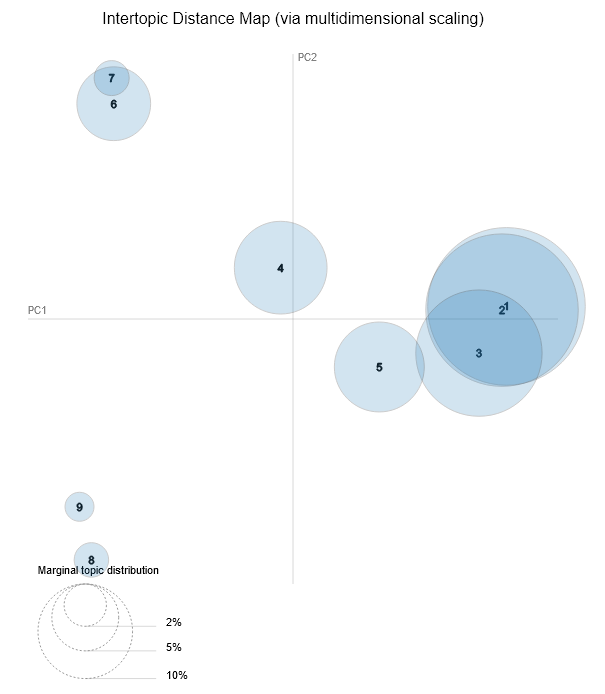
\includegraphics[width=1\columnwidth, scale=0.3]{images/topic_pca}}
\caption{Distanza tra i topic ottenuti}
\label{fig_topic_pca}
\end{figure}
Il grafico prodotto mostra dei topic abbastanza distribuiti e con poche sovrapposizioni, che sono comunque giustificate considerando la similarità intrinseca dei topic in oggetto.
Visualizzando le parole più frequenti all'interno dei topic si è cercato di assegnare il sottogenere musicale associato ad ogni topic, i risultati sono mostrati in tabella \ref{t_topic_label}.
\begin{table}[H]
\centering
\caption{Top 10 parole frequenti per topic}
\resizebox{\columnwidth}{!}{
\begin{tabular}{|l||llllllllll||l|}
\hline
id & \multicolumn{1}{l|}{} & \multicolumn{1}{l|}{} & \multicolumn{1}{l|}{} & \multicolumn{1}{l|}{} & \multicolumn{1}{l|}{} & \multicolumn{1}{l|}{} & \multicolumn{1}{l|}{} & \multicolumn{1}{l|}{} & \multicolumn{1}{l|}{} &      & Potential topic \\ \hline
1        & ey                    & dark                  & night                 & fal                   & light                 & dream                 & soul                  & heart                 & sky                   & cold & Death           \\ \hline
2        & tim                   & nev                   & know                  & see                   & feel                  & way                   & lik                   & com                   & lov                   & lif  & Doom            \\ \hline
3        & lif                   & die                   & dead                  & lie                   & kil                   & pain                  & fuck                  & mind                  & hat                   & liv  & Thrash          \\ \hline
4        & blood                 & burn                  & hel                   & fir                   & dea                   & shal                  & black                 & com                   & sin                   & flam & Black           \\ \hline
5        & god                   & war                   & man                   & evil                  & land                  & pow                   & new                   & ear                   & nam                   & rid  & Power           \\ \hline
6        & on                    & tak                   & fre                   & stand                 & ris                   & high                  & break                 & hand                  & watch                 & play & Heavy           \\ \hline
7        & fight                 & got                   & get                   & strength              & right                 & along                 & emot                  & big                   & wear                  & chas & Progressive     \\ \hline
8        & hard                  & yeah                  & dant                  & sing                  & song                  & rock                  & anyth                 & dog                   & wom                   & bal  & Rock            \\ \hline
9        & gold                  & welcom                & doom                  & sev                   & tal                   & wint                  & strange               & snow                  & hous                  & sink & Folk            \\ \hline
\end{tabular}
}
\label{t_topic_label}
\end{table}
Alcuni topic sono facilmente identificabili grazie alla conoscenza del dominio, parole come "god", "land" o "power" sono facilmente ricollegabili al Power metal, mentre per generi come il Death o il Doom i risultati prodotti sono piuttosto ambigui. Per ottenere un'indicazione più rigorosa riguardo la bontà dei risultati vengono calcolate le misure di Perplexity e Topic Coherence (variante sliding window) con valori rispettivamente pari a -6.5242 e 0.3978.
\section{Classificazione}
La classificazione segue due procedimenti distinti nel caso di singola label o di label multipla. In comune vi è il fatto che il dataset viene suddiviso in 80\% training e 20\% test nello stesso modo per garantire consistenza ai risultati prodotti.
\subsection{Classificazione multi-label}
\subsubsection{Labeled LDA}
Il primo modello utilizzato per la classificazione multi-label è un LLDA, la scelta di utilizzare un algoritmo di questo tipo è evidente, il semplice LDA, essendo un algoritmo non supervisionato non si presta bene per una classificazione di questo tipo, inoltre ogni lirica è etichettata e questo ci porta a ragionare in termini di classificazione supervisionata piuttosto che non. Rispetto al tradizionale approccio utilizzato da LDA, questo tipo di algoritmo restringe la distribuzione delle parole invece che su tutti i topic, solamente su quelli che rispettano l'etichetta presente nel training set. Questo vincolo è mostrato in maniera grafica in figura \ref{fig_llda}.

\begin{figure}[H]
\vspace{-5mm}
  \begin{subfigure}[b]{0.45\textwidth}
  \centering
    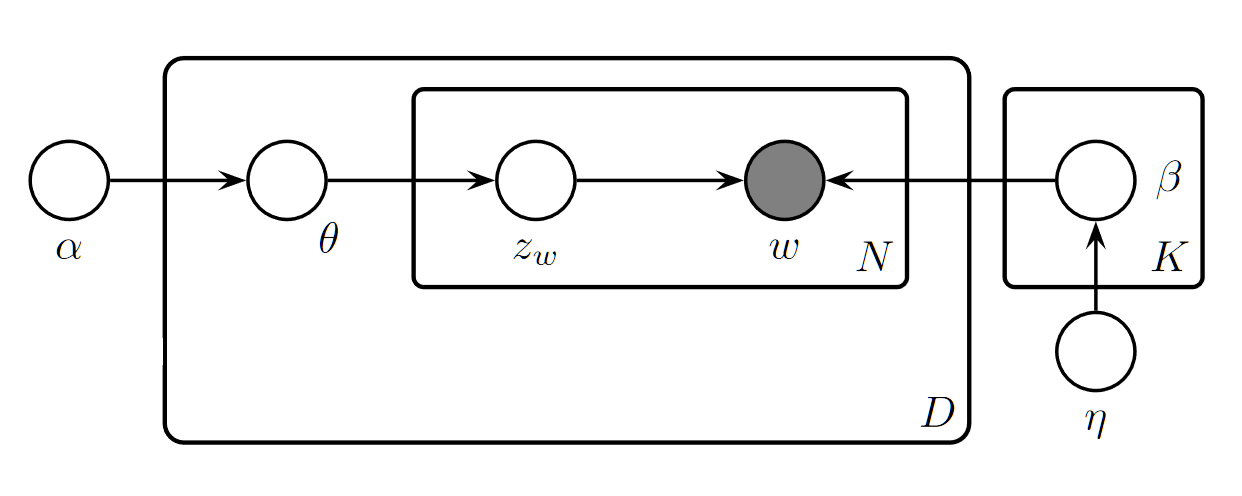
\includegraphics[width=0.7\textwidth]{images/lda}
    \caption{LDA tradizionale}
  \end{subfigure}
  %
   \hfill
  \begin{subfigure}[b]{0.45\textwidth}
  \centering
    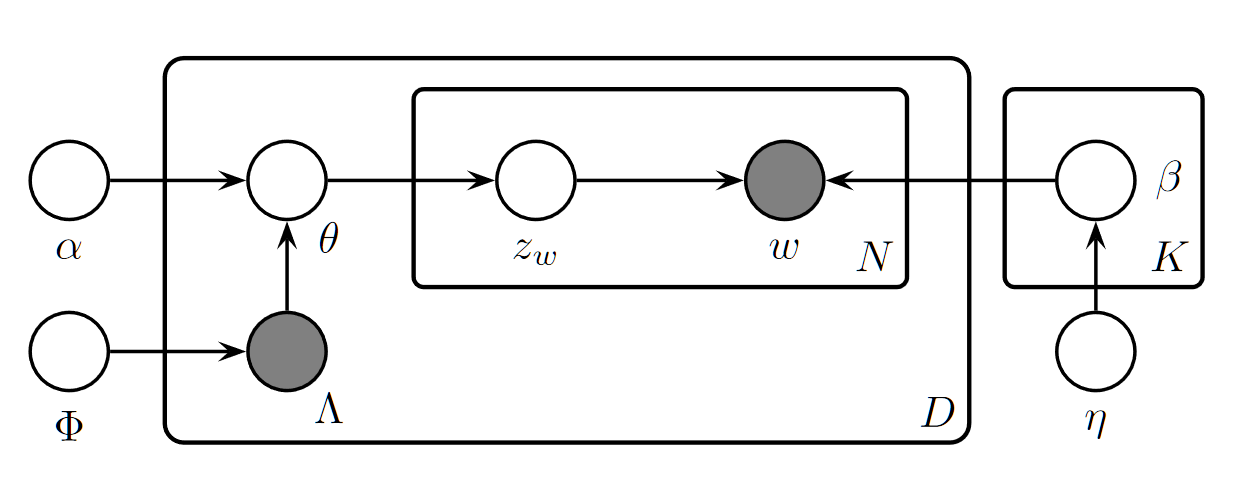
\includegraphics[width=0.7\textwidth]{images/llda}
    \caption{Labeled LDA}
  \end{subfigure}
  \caption{Differenza tra modello non supervisionato e supervisionato}
  \label{fig_llda}
\end{figure}
Il modello presenta una minima differenza con LDA, il training ed il testing vengono eseguiti utilizzando un campionamento di Gibbs collassato, esattamente come accade per il modello tradizionale. Il modello viene addestrato per 100 epoche, con parametri $ \alpha = 0.1 / 9 $ e $ \beta = 1 $. La scelta dei parametri è influenzata dal fatto che un valore piccolo di $ \alpha $ dovrebbe portare il modello a classificare più frequentemente i campioni con pochi topic contemporaneamente, inoltre dai test sperimentali è la combinazione di parametri che ottiene la likelihood migliore sui dati.
Le metriche utilizzate per la valutazione sono le classiche Micro-average, Macro-average e due metriche pensate per task di questo tipo ovvero la Hamming-loss e la Exact Match Ratio. La prima è definibile come la frazione di label non correttamente classificate:
\begin{equation}
HL=\frac{1}{|N|*|L|}\sum_{i=1}^{|N|}\sum_{j=1}^{|L|}xor(y_ij, z_ij)
\end{equation}
Ed è utile per verificare se il modello non sta classificando in maniera completamente casuale, la seconda invece verifica il numero di multilabel perfettamente classificate:\\
\begin{equation}
EMR = \frac{1}{|N|}\sum_{i=1}^{|N|}I(Y_i = Z_i)
\end{equation}
I risultati sono riportati in tabella \ref{t_res_llda}:\\
\begin{table}[H]
\centering
\caption{Risultati LLDA}
\begin{tabular}{|l|l|l|l|}
\hline
\textbf{F1-Mi} & \textbf{F1-Ma} & \textbf{HL} & \textbf{EMR} \\ \hline
0.3300         & 0.3200         & 0.3158      & 0.0318       \\ \hline
\end{tabular}
\label{t_res_llda}
\end{table}
Come ci si aspettava i risultati sono molto bassi, il dataset è complesso ed estremamente sbilanciato, questo è abbastanza per giustificare il fallimento del modello. E' relativamente buono il valore della $ HL $, il modello sembra apprendere delle differenze sensate, l'EMR mostra invece come non sia praticamente mai in grado di ottenere una classificazione perfetta di tutte le label correttamente.
\subsubsection{Percettrone multistrato}
Un altro modello utilizzato in letteratura per la classificazione multi-label è il percettrone multistrato (MLP), l'architettura scelta è stata ottenuta in maniera sperimentale ed è così definita (Tabella \ref{t_mlp_arch}):
\begin{table}[H]
\centering
\caption{Architettura MLP}
\begin{tabular}{|l|l|l|}
\hline
\textbf{Layer} & \textbf{Output} & \textbf{Param \#} \\ \hline
dense (Dense)         & (None, 256)           & 334336            \\ \hline
dropout (Dropout)     & (None, 256)           & 0                 \\ \hline
dense\_1 (Dense)      & (None, 128)           & 32896             \\ \hline
dense\_2 (Dense)      & (None, 9)             & 1161              \\ \hline
\end{tabular}
\label{t_mlp_arch}
\end{table}
Il modello viene addestrato per 30 epoche utilizzando l'ottimizzatore Adam ($ lr = 0.01 $) con riduzione del learning rate di un fattore $ \phi = 0.1 $ in caso di non decrescita della loss sul test set.
I risultati ottenuti sono decisamente migliori come illustrato in tabella \ref{t_res_mlp}.
\begin{table}[H]
\centering
\caption{Risultati MLP}
\begin{tabular}{|l|l|l|l|}
\hline
\textbf{F1-Mi} & \textbf{F1-Ma} & \textbf{HL} & \textbf{EMR} \\ \hline
0.4300         & 0.3200         & 0.1493      & 0.2493       \\ \hline
\end{tabular}
\label{t_res_mlp}
\end{table}
Particolarmente interessante il valore molto basso della Hamming-Loss, inoltre in questo caso un buon 25\% delle label viene perfettamente classificato.

\subsection{Classificazione singola-label}
In questa sezione vengono descritti i risultati ottenuti applicando diversi algoritmi supervisionati per 
% Please add the following required packages to your document preamble:
% \usepackage[normalem]{ulem}
% \useunder{\uline}{\ul}{}

\section*{References}

Please number citations consecutively within brackets \cite{b1}. The 
sentence punctuation follows the bracket \cite{b2}. Refer simply to the reference 
number, as in \cite{b3}---do not use ``Ref. \cite{b3}'' or ``reference \cite{b3}'' except at 
the beginning of a sentence: ``Reference \cite{b3} was the first $\ldots$''

Number footnotes separately in superscripts. Place the actual footnote at 
the bottom of the column in which it was cited. Do not put footnotes in the 
abstract or reference list. Use letters for table footnotes.

Unless there are six authors or more give all authors' names; do not use 
``et al.''. Papers that have not been published, even if they have been 
submitted for publication, should be cited as ``unpublished'' \cite{b4}. Papers 
that have been accepted for publication should be cited as ``in press'' \cite{b5}. 
Capitalize only the first word in a paper title, except for proper nouns and 
element symbols.

For papers published in translation journals, please give the English 
citation first, followed by the original foreign-language citation \cite{b6}.

\begin{thebibliography}{00}
\bibitem{b1} G. Eason, B. Noble, and I. N. Sneddon, ``On certain integrals of Lipschitz-Hankel type involving products of Bessel fsdasdaunctions,'' Phil. Trans. Roy. Soc. London, vol. A247, pp. 529--551, April 1955.
\bibitem{b2} J. Clerk Maxwell, A Treatise on Electricity and Magnetism, 3rd ed., vol. 2. Oxford: Clarendon, 1892, pp.68--73.
\bibitem{b3} I. S. Jacobs and C. P. Bean, ``Fine particles, thin films and exchange anisotropy,'' in Magnetism, vol. III, G. T. Rado and H. Suhl, Eds. New York: Academic, 1963, pp. 271--350.
\bibitem{b4} K. Elissa, ``Title of paper if known,'' unpublished.
\bibitem{b5} R. Nicole, ``Title of paper with only first word capitalized,'' J. Name Stand. Abbrev., in press.
\bibitem{b6} Y. Yorozu, M. Hirano, K. Oka, and Y. Tagawa, ``Electron spectroscopy studies on magneto-optical media and plastic substrate interface,'' IEEE Transl. J. Magn. Japan, vol. 2, pp. 740--741, August 1987 [Digests 9th Annual Conf. Magnetics Japan, p. 301, 1982].
\bibitem{b7} M. Young, The Technical Writer's Handbook. Mill Valley, CA: University Science, 1989.
\end{thebibliography}
\vspace{12pt}
\color{red}
IEEE conference templates contain guidance text for composing and formatting conference papers. Please ensure that all template text is removed from your conference paper prior to submission to the conference. Failure to remove the template text from your paper may result in your paper not being published.

\end{document}
